% !TeX root = RJwrapper.tex
\title{survivalSL: an R Package for Predicting Survival by a Super Learner}


\author{by Camille Sabathe and Yohann Foucher}

\maketitle

\abstract{%
The R package \pkg{survivalSL} contains a variety of functions to construct a super learner in the presence of censored times-to-event and to evaluate its prognostic capacities. Compared to the available packages, we propose additional learners, loss functions for the parameter estimations, and user-friendly functions for evaluating prognostic capacities and predicting survival curves from new observations. We performed simulations to describe the value of our proposal. We also detailed its usage by an application in multiple sclerosis. Because machine learning is increasingly being used in predictive studies with right-censoring, we believe that our solution can be useful for a large community of data analysts, beyond this clinical application .
}

\let\proglang=\textsf
\newcommand{\class}[1]{'\code{#1}'}
\newcommand{\fct}[1]{\code{#1()}}
\newcommand{\deriv}{\mathrm{d}}
\newcommand{\prob}{\mathbb{P}}
\newcommand{\loss}{\mathrm{L}}
\newcommand{\ic}{$\mathrm{IC}_{95\%}$}
\newcommand{\transp}{^{\top}}
\newcommand{\esp}{\mathbb{E}}
\newcommand{\indic}{\mathbb{1}}
\newcommand{\argmin}{\mathop{\mathrm{argmin}}}
\newcommand{\argmax}{\mathop{\mathrm{argmax}}}

\hypertarget{introduction}{%
\section{Introduction}\label{introduction}}

In clinical practice, the prediction of the probability that a subject will experience an event is often of interest. For instance, for patients with multiple sclerosis under first-line treatment, the prediction of disease progression would result in the early identification of non-responders and help in deciding the switch to second-line treatment. However, the time-to-disease progression is often not observable for all subjects because of a lack of follow-up, i.e., right-censoring.

Several regressions can be used for prediction from right-censored data. The most popular is probably the proportional hazards (PH) model \citep{cox_regression_1972}. The corresponding baseline hazard function can be obtained by assuming parametric distributions \citep{andersenCountingProcessModels1985}, nonparametric estimators \citep{linBreslowEstimator2007} or other flexible approaches such as splines \citep{rosenbergHazardFunctionEstimation1995}. Penalized PH models have also been proposed, particularly useful for high-dimensional data \citep{goemanPenalizedEstimationCox2009}. The accelerated failure times (AFT) approach also constitutes an alternative to the PH assumption \citep{wei_accelerated_1992}.

In parallel to these regression-based methods, machine learning is increasingly used. Support-vector machines \citep{shivaswamySupportVectorApproach2007}, neural networks \citep{faraggiNeuralNetworkModel1995}, or even random forests \citep{ishwaranRandomSurvivalForests2008a} have been successfully developed for censored time-to-event data. Ensemble learning allows us to combine regressions and algorithms by minimizing the cross-validated loss function \citep{breimanStackedRegressions1996}. SL was first proposed by \citet{vanderlaanSuperLearner2007} and \citet{vanderlaandudoit2003} from the theory of unified loss-based estimation.

\citet{polleyChapterSuperLearning2011} and \citet{polleyChapter16Super2011} extended the SL to right-censored data. Two \texttt{R}-based solutions are available on GitHub repositories. The \pkg{SuperLearner-Survival} repository is related to the work by \citet{golmakaniSuperLearnerSurvival2020a}. It allows us to obtain the linear predictor of a PH regression. The \pkg{survSuperLearner} package was developed by \citet{westlingPkgsurvSuperLearnerSuperLearning2021} with additional learners: several parametric PH models (Exponential, Weibull, log-logistic, and piecewise constant hazard), generalized additive Cox regression, and random survival forest.

In this paper, we aim to extend these solutions by i) additional learners (accelerated failure times, neural networks, penalized regressions), ii) several loss functions for the estimation of the parameters (Brier score, negative binomial log-likelihood, etc.) and iii) user-friendly S3 methods for evaluating the predictive capacities, as well as predicting survival curves from new observations (Section 1). In the second section, we propose a simulation-based study to compare the performances of our proposal with that of the alternative solutions. In the third section, we detail its usage by an application in multiple sclerosis. Finally, we discuss the strengths, weaknesses and perspectives of our solution.

\hypertarget{methods}{%
\section{Methods}\label{methods}}

\hypertarget{notations}{%
\subsection{Notations}\label{notations}}

For a subject \(i\) in a sample of \(N\) independent subjects \((i=1,...,N)\), we denoted the time-to-event by \(T_i^\star\). Right-censoring leads the observation of \(T_i=\min(T_i^\star, C_i)\), where \(C_i\) is the censoring time. Let \(D_i= \mathbb{1}\left \lbrace T_i^\star \leq C_i \right \rbrace\) be the event indicator. The survival function at time \(t\) for a subject with the characteristics \(Z_i\) at baseline is defined by \(S(t \mid Z_i ) = \mathbb{P}(T_i^\star> t \mid Z_i)\).

\hypertarget{definition-of-the-super-learner}{%
\subsection{Definition of the super learner}\label{definition-of-the-super-learner}}

Let \(S_{sl}(.)\) be the survival function obtained by the SL such as \(S_{sl}(t \mid Z_i)=\sum_{m=1}^M w_m \times S_m(t \mid Z_i)\), where \(S_m(.)\) is the survival function obtained by its \(m\)th learner (\(m = 1,...,M\)), and \(w = (w_1,...,w_M)\) are the corresponding weights with respect to \(\sum_1^M w_m=1\) and \(0 \leq w_m \leq 1\). The estimations of the learners and the weights can be obtained by respecting the following steps \citep{Polley2010}:

\begin{enumerate}
\def\labelenumi{\arabic{enumi}.}
\item
  Estimate the \(M\) models or algorithms on the entire sample as usual. The procedure of estimation can be different for each model. For instance, a parametric model may be fitted by maximizing the full likelihood, a Cox regression by maximizing the partial likelihood and estimating the baseline survival function with Breslow method, or a random survival forest by maximizing the between-node survival differences according to the log-rank statistic.
\item
  By using the \(M\) models or algorithms estimated in the step \#1 (\(m=1,...,M\)), predict the values \(\hat{S}_m(u \mid Z_i)\) for each subject \(i=1, ...,N\) and for a vector of \(U\) times (\(u = u_1, ..., u_U\)) and stack the values in a 3-dimensional array of size (\(N\) \(\times\) \(U\) \(\times\) \(M\)).
\item
  Split the sample into a training and validation sample according to a V-fold cross-validation, i.e., \(V\)-equal size and randomly selected groups. Let \(T(v)\) be the \(v\)th training sample and \(V(v)\) be the corresponding validation sample (\(v = 1, .., V\)).
\item
  For the \(v\)th fold, estimate the \(M\) models or algorithms from \(T(v)\). The learners based on the estimation of hyperparameters should be tuned for each of the \(V\) folds. Note that this tunning step is often based on cross-validation and should be performed for each of the \(V\) folds. Regarding the corresponding computational burden, a compromise consists of using the hyperparameters estimated at the step \#1 \citep{florent2021}.
\item
  Compute the corresponding predicted survival rates for the individuals of the validation sample \(V(v)\) and the \(U\) times.
\item
  Stack the predictions \(\tilde{S}_m(u \mid Z_i)\) obtained in the step \#5 in a 3-dimensional array of size (\(N\) \(\times\) \(U\) \(\times\) \(M\)).
\item
  Determine the loss function \(\mathbb{L} (w \mid \tau)\) for quantifying the gap of the predictions \(\tilde{S}_{sl}( \tau \mid Z_i) = \sum_{m=1}^M w_m \tilde{S}_m(\tau \mid Z_i)\) and the observations \((T_i, D_i)\) for a prognostic up to \(\tau\). The loss functions available in the package are listed in the next subsection.
\item
  Estimate the weights \(w\) by minimizing the loss function for a prognostic up to a time \(\tau\):
\end{enumerate}

\[\hat{w} = \underset{w}{\mathrm{arg \; min}} \; \mathbb{L} (w \mid \tau)\]

\begin{enumerate}
\def\labelenumi{\arabic{enumi}.}
\setcounter{enumi}{8}
\tightlist
\item
  Combine \(\hat{w}_m\) with \(\hat{S}_m(u \mid Z_i)\) to obtain the final super learner:
\end{enumerate}

\[\hat{S}_{sl}(t \mid Z_i) = \sum_{m=1}^M \hat{w}_m \hat{S}_m(t \mid Z_i)\]

\hypertarget{available-loss-functions-for-estimating-the-weights}{%
\subsection{Available loss functions for estimating the weights}\label{available-loss-functions-for-estimating-the-weights}}

Several loss functions \(\mathbb{L} (w \mid \tau)\) are available in the package. The Brier score (BS) for right-censored data and a prediction at time \(\tau\) is defined by:
\[BS(w \mid \tau) = \frac{1}{N}  \sum_{i} \left [ \frac{ \tilde{S}_{sl}( \tau \mid Z_i)^2 \mathbb{1} \lbrace T_i \leq \tau, D_i=1  \rbrace  }{ \hat{G}(T_i) } +   \frac{ ( 1-\tilde{S}_{sl}( \tau \mid Z_i))^2 \mathbb{1} \lbrace T_i>\tau  \rbrace } { \hat{G}(\tau) } \right ]\]
where \(\hat{G}(u)=\mathbb{P}(C_i > u)\) is the survival function of the censoring time \citep{houwelingenDynamicPredictionClinical2012a}. The corresponding \(\tau\)-restricted integrated BS is \(RIBS(w \mid \tau) = \int_0^{\tau} BS(u) du\). The integrated BS equals \(RIBS(w \mid \max(T_i^\star))\). We also considered the negative binomial log-likelihood (BLL), which is defined for a prognostic at time \(\tau\) as follows:
\[BLL(w \mid \tau) = \frac{1}{N} \sum_{i} \left[  \frac{ \log (1-\tilde{S}_{sl}( \tau \mid Z_i) ) \mathbb{1} \lbrace T_i \leq \tau,D_i=1 \rbrace } {\hat{G}(T_i)} + \frac{ \log ( \tilde{S}_{sl}( \tau \mid Z_i) ) \mathbb{1} \lbrace T_i>\tau \rbrace } { \hat{G}(\tau) }\right]\]
We also proposed the corresponding integrated and \(\tau\)-restricted integrated versions. Additionally, we implemented the concordance index (CI) as defined by \citet{uno_c-statistics_2011}:
\[CI(w \mid \tau) = \frac{\sum_{i}\sum_{j} \mathbb{1} \lbrace T_j < T_i , \tilde{S}_{sl}( \tau \mid Z_j) > \tilde{S}_{sl}( \tau \mid Z_i)  \rbrace D_j}{ \sum_{i}\sum_{j} \mathbb{1} \lbrace T_j < T_i \rbrace D_j }\]
Finally, we considered the area under the time-dependent ROC curve, i.e., the sensitivity (SE) against one minus the specificity (SP) at each threshold \(\eta\) \citep{hung_estimation_2010}:

\[ SE_\eta(w \mid \tau) = \frac{ \sum_i D_i \mathbb{1}\lbrace T_i \leq \tau , \tilde{S}_{sl}( \tau \mid Z_i) > \eta \rbrace / (1 - \hat{G}(T_i)) }{ \sum_i D_i \mathbb{1}\lbrace T_i \leq \tau \rbrace / (1 - \hat{G}(T_i))}\]
\[SP_\eta(w \mid \tau) = \frac{ \sum_i  \mathbb{1}\lbrace T_i > \tau , \tilde{S}_{sl}( \tau \mid Z_i) \leq \eta \rbrace }{ \sum_i \mathbb{1}\lbrace T_i > \tau \rbrace } \]

\hypertarget{available-learners}{%
\subsection{Available learners}\label{available-learners}}

Several models or algorithms are proposed in the \pkg{survivalSL} package:

\begin{itemize}
\item
  \texttt{Parametric\ AFT\ models.} They can be considered with Weibull, Gamma or generalized Gamma distributions (\pkg{flexsurv} package). The parameters are estimated by likelihood maximization.
\item
  \texttt{Parametric\ PH\ models.} They can be considered with Exponential or Gompertz distributions (\pkg{flexsurv} package). The parameters are estimated by likelihood maximization.
\item
  \texttt{Spline-based\ PH\ models.} We considered the spline-based survival model proposed by \citet{royston_flexible_2002}. To estimate the baseline distribution, it involves one hyperparameter: the number of internal knots of the natural cubic spline, with a default grid search \(k = \left \lbrace 1, 2, 3, 4 \right \rbrace\). The parameters are estimated by likelihood maximization (\pkg{flexsurv} package).
\item
  \texttt{Semi-parametric\ PH\ models.} It corresponds to a PH model (\pkg{coxph} function of the \pkg{survival} package) with a non-parametric baseline hazard function estimated by using the Breslow estimator \citep{linBreslowEstimator2007}. This approach can be used with or without a forward selection of covariates by using the AIC.
\item
  \texttt{Penalized\ PH\ models.} For high-dimensional data and/or covariate selection, three penalties can be used for the previous semiparametric PH model: Lasso, Ridge, or Elastic-Net (\pkg{glmnet} package). The quantitative covariates are transformed with B-splines to relax the log-linear assumption. The hyperparameters \(\lambda\) of the Lasso regression allows for selection of the covariates, while it allows for the shrinkage of the regression coefficients in the Ridge regression. The Elastic-Net allows the two penalties. By default, we implemented the grid search proposed by \citet{simon_2011_ElasticNet_Cox} for \(\lambda\) and \(\left \lbrace 0.1, 0.2, ..., 0.9 \right \rbrace\) for \(\alpha\). The Lasso penalization corresponds to \(\alpha=0\), while the Ridge penalization corresponds to \(\alpha=1\).
\item
  \texttt{Random\ survival\ forests.} This ensemble tree method extends Breiman's random forest framework to right-censored data \citep{ishwaranRandomSurvivalForests2008a}. It allows estimation of the cumulative hazard function in each node by using the nonparametric estimator of survival proposed by \citet{aalen1979}. It involves three hyperparameters (\pkg{randomSRC} package): number of covariates to test for splitting the node, minimal number of events per terminal node, and number of trees. The default grid search is \texttt{mtry} = \(\left \lbrace 1,2,...,2+0.5\times \textrm{number of covariates} \right \rbrace\), \texttt{nodesize} \(= \left \lbrace 2, 4, 6, 10, 20, 30, 50, 100 \right \rbrace\) and \texttt{ntree} \(= 500\), respectively.
\item
  \texttt{Survival\ neural\ networks.} We implemented the method proposed by \citet{biganzoli_feed_1998}. It allows using the \pkg{nnet} package for estimating a feed forward neural network model for partial logistic regression. It involves four hyperparameters: the length of the time intervals, the number of units in the hidden layer, the weight decay, the maximum number of iterations, and the maximum allowable number of weights. The optimal combination is estimated by cross-validation and the previous possible loss functions. The default grid search is composed by \texttt{inter} \(= 1\), \texttt{size} \(= \left \lbrace 2, 4, 6, 8, 10 \right \rbrace\), \texttt{decay} \(= \left \lbrace 0.001, 0.01, 0.02, 0.05 \right \rbrace\), \texttt{maxit} \(= 100\), and \texttt{MaxNWts} \(= 10000\), respectively.
\end{itemize}

\hypertarget{simulations}{%
\section{Simulations}\label{simulations}}

\hypertarget{design}{%
\subsection{Design}\label{design}}

We simulated 1000 data sets for each scenario. The times-to-event were generated from Weibull distributions with PH assumption. The censoring times were generated from uniform distributions to obtain a 40\% censoring rate. We studied two sample sizes for learning (200 and 500), while the validation samples were composed of 500 subjects. We proposed two contrasting scenarios (Figure \ref{fig:scenarios} in Appendix):

\begin{itemize}
\item
  A simple scenario with 6 independent covariates, 2 were continuous and 4 qualitative. Among them, 1 continuous and 2 qualitative covariates were associated with the times-to-event distribution without any log-linearity issue.
\item
  A complex scenario with 23 correlated covariates: 12 continuous covariates (several nonlinear relationships, two effects were step functions, two were quadratic functions, five were log-linear), 11 qualitative covariates and 1 interaction.
\end{itemize}

We compared our proposed SL with each included learner, the perfectly specified PH model (i.e., the model used to generate the times-to-event, the only estimation consisting of the regression coefficients), and the SL obtained by the \pkg{survSuperLearner} package \citep{westlingPkgsurvSuperLearnerSuperLearning2021}. We decided to use the package proposed by \citet{westlingPkgsurvSuperLearnerSuperLearning2021} as a comparator because it includes additional learners compared to the functions proposed by \citet{golmakaniSuperLearnerSurvival2020a}. The SL weights were estimated by minimizing the integrated BS (IBS) for all the methods.

In the SL proposed by \citet{westlingPkgsurvSuperLearnerSuperLearning2021}, we included the 5 possible learners: the PH model with the Breslow estimator, the Exponential PH model, the random survival forests, the Lasso PH model and the PH model with the univariate selection of covariates (\(p<0.05\)). We used the default grid of the hyperparameters.

In our proposed SL, we included the 7 possible learners: the PH model with the Breslow estimator, the same model with forward selection based on AIC minimization, the Elastic-Net PH model with B-splines on quantitative covariates, the random survival forest, the Exponential PH model, the Gamma distribution-based AFT model, and the survival neural network. Note that we did not consider the Weibull PH model since it was used for data generation. We used the default grid of the hyperparameters.

\hypertarget{results-of-the-simple-scenario}{%
\subsection{Results of the simple scenario}\label{results-of-the-simple-scenario}}

Figure \ref{fig:ibs-scea-ggplot} presents the distributions of the IBS over the learning (on the left) and validation samples (on the right). The related \texttt{R} code is available in Appendix. Consider the situation where \(N=200\) for learning and \(N=500\) for validation (the first two plots on the top). The perfectly specified model had the lower IBS. This result was expected since it constitutes the gold standard to reach by the other methods. The Elastic-Net PH regression outperformed all the other approaches in the learning samples. This result explained the important weight of this method, approximately 25\% in our SL, as illustrated in Figure \ref{fig:wscea-ggplot} in Appendix. Nevertheless, this apparent result was not observed in the validation samples, illustrating overfitting.

In both the learning and the validation samples, our proposed SL, the PH model with the Breslow estimator, and the same model with forward selection based on the AIC had the best performances, higher than that of the SL proposed by \citet{westlingPkgsurvSuperLearnerSuperLearning2021}.

The survival neural network and the PH model with an Exponential distribution were associated with larger values of the IBS in both the learning and the validation samples. Comparatively, the results were closed across the other methods. In the validation samples, the highest variability of the IBS was observed for the survival neural network.

\begin{figure}

{\centering 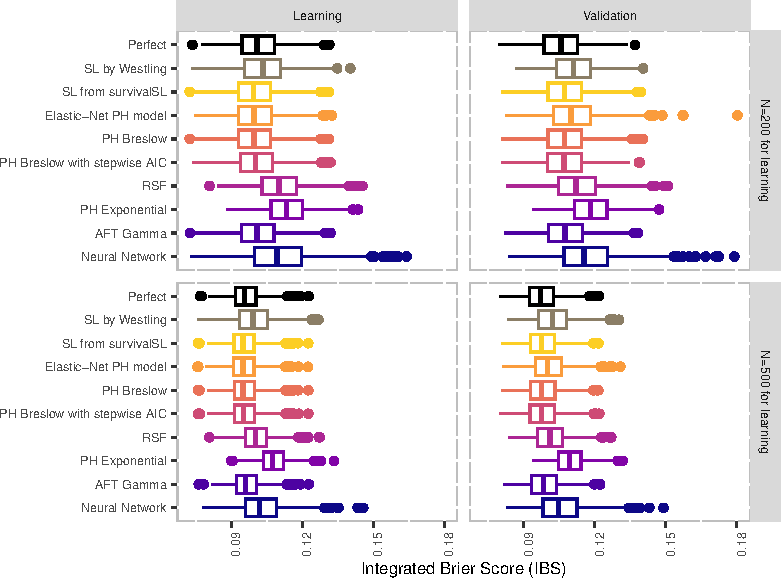
\includegraphics{RJ-2024-037_files/figure-latex/ibs-scea-ggplot-1} 

}

\caption{Simulation results in the simple context.}\label{fig:ibs-scea-ggplot}
\end{figure}

When \(N=500\) in both the learning and the validation samples (the two bottom plots of Figure \ref{fig:ibs-scea-ggplot}), the results were close. However, one can note that the means and variances of the IBS were lower.

\hypertarget{results-of-the-complex-scenario}{%
\subsubsection{Results of the complex scenario}\label{results-of-the-complex-scenario}}

The related \texttt{R} code is available in Appendix. As illustrated in Figure \ref{fig:ibs-sceb-ggplot}, regarding the results in the validation samples, our proposed SL and the Elastic-Net PH regression outperformed the other models/algorithms. More precisely, the mean of the IBS was lower for the Elastic-Net PH model for a learning sample size of 200. The value of our proposed SL was close. When \(N=500\) for learning, the mean of the IBS was lower for our SL, but that of the Elastic-Net PH model was close. Nevertheless, regardless of the sample size for learning, our SL was associated with lower variance in the IBS.

Among the other differences compared to the simple context, the random survival forests and the survival neural networks performed better than the other model-based predictors, except the Elastic-Net PH model.

In both the learning and the validation samples, and regardless the sample size for learning, our proposed SL had slightly higher performances compared to the results of the SL proposed by \citet{westlingPkgsurvSuperLearnerSuperLearning2021}.

\begin{figure}

{\centering 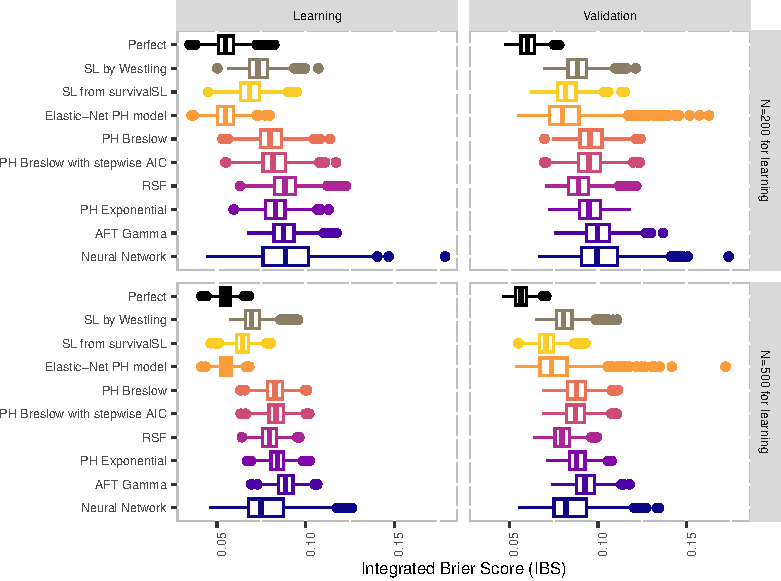
\includegraphics{RJ-2024-037_files/figure-latex/ibs-sceb-ggplot-1} 

}

\caption{Simulation results in the complex context.}\label{fig:ibs-sceb-ggplot}
\end{figure}

\hypertarget{running-times}{%
\subsection{Running times}\label{running-times}}

We further explored the time required to estimate a SL depending on the sample size and the number of predictors. For this purpose, we simulated data according to the complex scenario (Figure \ref{fig:scenarios} in Appendix). We used a 20-fold cross-validation, tested sample sizes from 500 to 3500, and reduced the number of predictors from 22 to 4. The results are illustrated by Figure \ref{fig:run-ggplot}. If we considered 20 predictors, the running times increased exponentially from 0.10 (\(N=500\)) to 3.23 hours (\(N=3500\)). For 10 predictors, the times increased from 0.06 to 1.67 hours.

\begin{figure}

{\centering 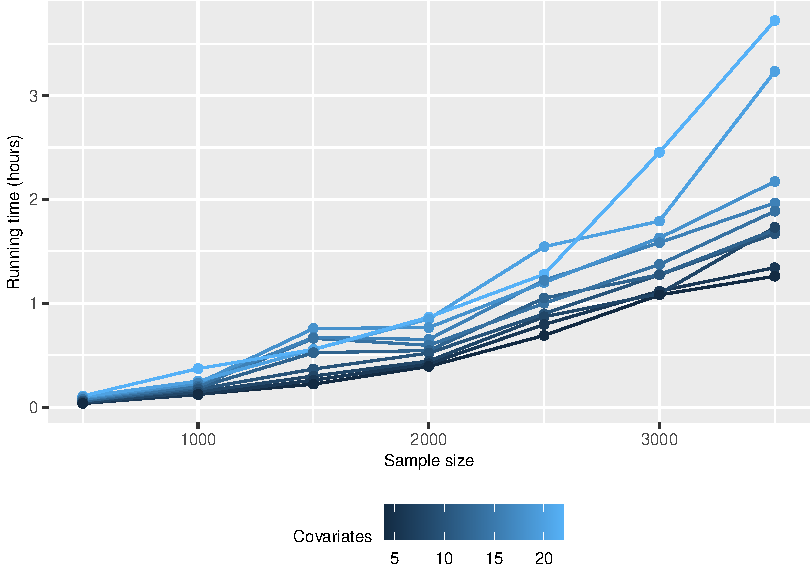
\includegraphics{RJ-2024-037_files/figure-latex/run-ggplot-1} 

}

\caption{Running times according to the sample size and the number of covariates. Results obtained for a MacBook Pro 2.6 GHz Intel Core i7 6 cores.}\label{fig:run-ggplot}
\end{figure}

\hypertarget{usage}{%
\section{Usage}\label{usage}}

\hypertarget{the-main-functions-of-the-package}{%
\subsection{The main functions of the package}\label{the-main-functions-of-the-package}}

The \texttt{survivalSL} function fits the SL. It is mainly based on the following arguments:

\begin{itemize}
\item
  \texttt{formula}: A formula object, with the response on the left, and the predictors on the right. The response must be a survival object as returned by the \texttt{Surv} function..
\item
  \texttt{methods}: The names of the learners included in the SL. At least two models/algorithms must be included. The complete list of candidates is described in Table \ref{tab:listemeth-tab-static}.
\item
  \texttt{data}: The data frame in which to look for the variables related to the follow-up time, the event indicator, and the covariates.
\item
  \texttt{metric}: The loss function used to estimate the weights of the learners.
\item
  \texttt{pro.time}: The prognostic time used for the Brier score, the negative binomial log-likelihood or the corresponding restricted versions.
\item
  \texttt{cv}: The number of cross-validated samples to estimate the weights of the learners.
\item
  \texttt{param.tune}: Optional list to define the grid search of the hyperparameter(s) or to set the value(s) of the hyperparameter(s). If \texttt{NULL}, the default grid is used.
\item
  \texttt{seed}: A numeric value for random seed for reproducibility. The default is \texttt{NULL}.
\end{itemize}

\begin{table}
\centering
\caption{\label{tab:listemeth-tab-static}List of possible learners (\#: Breslow's estimation of the baseline hazard function). The last column lists the learners included in the survSuperLearner proposed by Westling (2021). This package additionally considers generalized additive Cox regression and piecewise constant hazard regression.}
\centering
\fontsize{8}{10}\selectfont
\begin{tabular}[t]{l>{\raggedright\arraybackslash}p{8cm}l}
\toprule
Name & Description & Westling\\
\midrule
LIB\_COXall & Proportional hazards (PH) model with all covariates (\#) & Yes\\
LIB\_COXaic & PH model with covariate selection by AIC minimization (\#) & No\\
LIB\_COXen & PH model with B-spline for the quantitative covariates and Elastic-Net penalization (\#, hyperparameters: alpha and lambda) & Yes\\
LIB\_COXlasso & PH model with B-spline for the quantitative covariates and Lasso penalization (\#, hyperparameter: lambda) & Yes\\
LIB\_COXridge & PH model with B-spline for the quantitative covariates and Ridge penalization (\#, hyperparameter: lambda) & Yes\\
\addlinespace
LIB\_AFTgamma & Accelerated failure times (AFT) model with Gamma distribution & No\\
LIB\_AFTggamma & AFT model with generalized Gamma distribution & No\\
LIB\_AFTllogis & AFT model with log-logistic distribution & No\\
LIB\_AFTweibull & AFT model with Weibull distribution & Yes\\
LIB\_PHexponential & Parametric PH model with Exponential distribution & Yes\\
\addlinespace
LIB\_PHgompertz & Parametric PH model with Gompertz distribution & Yes\\
LIB\_PHspline & PH model with natural cubic spline as baseline distribution (hyperparameters: k) & No\\
LIB\_RSF & Random survival forest (hyperparameters: nodesize, mtry and ntree) & Yes\\
LIB\_PLANN & One-layer survival neural network (hyperparameters: n.nodes, decay, batch.size and epochs) & No\\
\bottomrule
\end{tabular}
\end{table}

Note that a method based on hyperparameters can be used several times with different values of hyperparameters. When the hyperparameters are specified by the user, the argument \texttt{param.tune} must be a list with their value(s) and name(s). For a user-friendly manipulation of the resulting \texttt{sltime} object, we proposed several S3 methods listed in Table \ref{tab:s3-tab-static}. They allow for evaluating the calibration and discrimination capacities, or predicting survival curves. These functions can be applied to new data sets. Similar S3 methods are available for other learners (\texttt{LIB\_AFTgamma}, \texttt{LIB\_COXlasso}, etc.).

\begin{table}
\centering
\caption{\label{tab:s3-tab-static}List of S3 functions applicable to an sltime object}
\centering
\fontsize{8}{10}\selectfont
\begin{tabular}[t]{l>{\raggedright\arraybackslash}p{11cm}}
\toprule
Function & Description\\
\midrule
plot.sltime & To obtain a calibration plot.\\
predict.sltime & To predict the survival probabilities from the SL and the included learners.\\
summary.sltime & To obtain metrics describing the prognostic capacities of the SL and the included learners.\\
print.sltime & To print the learners and their weights\\
\bottomrule
\end{tabular}
\end{table}

\hypertarget{application-to-multiple-sclerosis}{%
\subsection{Application to multiple sclerosis}\label{application-to-multiple-sclerosis}}

This section is not intended to propose guidelines for data analysis. It only consists of illustrating the use of the \pkg{survivalSL} package. Beside the present application, a recent work proposed recommendations for implementing such a SL \citep{phillips_practical_2023}.

The following application is related to the prediction of the time to disease progression from prognostic factors collected one year after the initiation of a first-line treatment, which is the baseline of the cohort (\(T^\star = 0\)). We also compared the prognostic capacities of the obtained SL with those of the modified Rio score \citep{sormaniScoringTreatmentResponse2013a}.

\texttt{Data\ description.} We detailed the implementation of the previous function with an application based on the OFSEP cohort, which was composed of 1300 simulated patients with multiple sclerosis. The simulations were performed from the observed cohort to obtain the present shared data set which complies with the General Data Protection Regulation of the European Union. More precisely, the prognostic factors were first simulated one by one, i.e., using the factors already simulated to obtain the next one. These simulations were based on linear or logistic models for continuous or categorical factors, respectively. Finally, the time to disease progression was simulated by a Weibull PH model, which explains why it was not considered among the learners.

\begin{verbatim}
library("survivalSL")
data(dataOFSEP); head(dataOFSEP)
\end{verbatim}

\begin{verbatim}
#>        time event age duration period gender relapse edss t1 t2 rio
#> 1 2.1195051     1  34     1113      0      1       1  low  0  0   1
#> 2 0.8160995     1  37     1296      0      1       1 high 1+  0   1
#> 3 1.9709546     1  33      995      1      1       0  low  0  0   0
#> 4 2.5881311     1  35      858      1      1       0  low  0  0   0
#> 5 1.4726224     1  31      759      1      0      2+ miss 1+  0   2
#> 6 1.6970962     1  40     1642      1      1       0 high  0  0   0
\end{verbatim}

The first two columns of the \texttt{dataOFSEP} table correspond to the time to disease progression (\texttt{time}) and the \texttt{event} indicator equals 1 for patients with events and 0 for right-censored patients. The time to disease progression was defined by the minimum among the time to first relapse, the time to increase of Expanded Disability Status Scale (EDSS), and the time to switch for inefficacy. The EDSS ranges from 0 to 10 (the higher levels of disability) and is based on an examination by a neurologist.

The other columns were the available predictors one year after the initiation of first-line therapy. The third and fourth columns were two quantitative predictors: patient \texttt{age} (in years) and disease \texttt{duration} (in days). The other columns were qualitative predictors: calendar \texttt{period} (1 if between 2014 and 2018, and 0 otherwise), \texttt{gender} (1 if women), diagnosis of \texttt{relapse} since treatment initiation (1 if at least one event, and 0 otherwise), and EDSS level (\texttt{miss} if missing, \texttt{low} if level between 0 and 2, and \texttt{high} otherwise). The variables \texttt{t1} and \texttt{t2} were related to the lesions observed from magnetic resonance imaging, namely, the new gadolinium-enhancing T1 lesion (\texttt{miss} if missing, \texttt{1+} if at least one lesion, and \texttt{0} otherwise) and the new T2 lesion (1 if at least one lesion, and 0 otherwise), respectively.

The last column corresponded to the modified Rio score, i.e., the sum of the relapses (0 for none, 1 for one event, and 2 for at least 2 events) and the new T2 lesion (0 for none, and 1 for at least one lesion) observed since the treatment initiation \citep{sormaniScoringTreatmentResponse2013a}. We transformed the categorical predictors into binary variables.

\begin{verbatim}
dataOFSEP$relapse.1 <- 1*(dataOFSEP$relapse=="1")
dataOFSEP$relapse.2 <- 1*(dataOFSEP$relapse=="2+")
dataOFSEP$edss.1 <- 1*(dataOFSEP$edss=="low")
dataOFSEP$edss.2 <- 1*(dataOFSEP$edss=="high")
dataOFSEP$t1.1 <- 1*(dataOFSEP$t1=="0")
dataOFSEP$t1.2 <- 1*(dataOFSEP$t1=="1+")
\end{verbatim}

\texttt{Super\ learner\ training.} We randomly selected two-thirds of the sample to train the SL, and the other third was further used for validation in the next subsection. We set the seed to ensure the results replicability.

\begin{verbatim}
set.seed(117)
dataOFSEP$train <- 1*rbinom(n=dim(dataOFSEP)[1], size=1, prob=2/3)
dataTRAIN <- dataOFSEP[dataOFSEP$train==1,]
dataVALID <- dataOFSEP[dataOFSEP$train==0,]
\end{verbatim}

We fitted the SL with the following learners: PH model with Gompertz baseline hazard function, AFT model with generalized Gamma distribution, Elastic-Net PH model with nonparametric baseline hazard function (Breslow estimator) and B-spline transformations of the quantitative variables, and random survival forest. We used the default grids to estimate the hyperparameters. The weights were estimated to minimize the concordance index at 2 years with a 30-fold cross-validation. Note that 851 patients were included in the training sample, and 651 events were observed. In such a situation, \citet{phillips_practical_2023} recommended at least 20 folds.

\begin{verbatim}
.f <- Surv(time, event) ~ age + duration + period + gender +
   relapse.1 + relapse.2 + edss.1 + edss.2 + t1.1 + t1.2
sl1 <- survivalSL(formula=.f, metric="uno_ci",  data=dataTRAIN,
      methods=c("LIB_COXen", "LIB_PHspline", "LIB_AFTggamma", "LIB_RSF"),
      cv=30, optim.local.min=TRUE, show_progress=FALSE, seed=117)
print(sl1, digits=4)
\end{verbatim}

\begin{verbatim}
#> The contribution of the learners: 
#> 
#>         leaners weights
#> 1     LIB_COXen  0.1775
#> 2  LIB_PHspline  0.2519
#> 3 LIB_AFTggamma  0.3039
#> 4       LIB_RSF  0.2667
#> 
#> Minimum of the 30-fold CV of the metric uno_ci:0.6851.
\end{verbatim}

Moreover, the package allows the user to propose a more precise grid for the hyperparameter-based methods. For instance for the spline-based PH model, the user may precise his/her own grid search:

\begin{verbatim}
.tune <- vector("list",4)
.tune[[2]] <- list(k=1:6)
sl2 <- survivalSL(formula=.f, metric="uno_ci",  data=dataTRAIN,
      methods=c("LIB_COXen", "LIB_PHspline", "LIB_AFTggamma", "LIB_RSF"),
      cv=30, optim.local.min=TRUE, param.tune=.tune, show_progress=FALSE, seed=117)
print(sl2, digits=4)
\end{verbatim}

\begin{verbatim}
#> The contribution of the learners: 
#> 
#>         leaners weights
#> 1     LIB_COXen  0.2486
#> 2  LIB_PHspline  0.3340
#> 3 LIB_AFTggamma  0.1773
#> 4       LIB_RSF  0.2401
#> 
#> Minimum of the 30-fold CV of the metric uno_ci:0.684.
\end{verbatim}

On a MacBook Pro 2.6 GHz Intel Core i7 6 cores, the running times to estimate \texttt{sl1} and \texttt{sl2} were 11.0 and 13.2 minutes, respectively. Note that the optional argument related to the definition of the grid may be used to estimate the hyperparameters from the entire sample and use the related values in each fold of the steps \#4 and \#5 of the super learner estimation. This strategy may be associated with overfitting, but an important decrease in the computation time and the fluctuation of the results. Indeed, regarding the random allocation of the individuals in the folds at the steps \#1 (for estimating the learners from the entire training sample) and \#3 (for estimating the prediction matrix includes in the loss function), the results depend on the generating pseudo random numbers. To illustrate this fluctuation, the \texttt{sl2} estimation was performed for several seeds in Appendix. The weights of the learners significantly varied but the predictive performances of the super learners were stable.

\texttt{Super\ learner\ validation.} We further studied the prognostic capacities of this algorithm, always up to 2 years. First, we observed that the metrics between the training and validation samples were close, illustrating the absence of overfitting.

\begin{verbatim}
rbind(train = summary(sl2, method="sl", pro.time=2, digits=4)$metrics,
      test =  summary(sl2,  newdata=dataVALID, method="sl",
                      pro.time=2, digits=4)$metrics)
\end{verbatim}

\begin{verbatim}
#>         p_ci uno_ci    auc     bs    ibs   ribs    bll ibll ribll        ll
#> train 0.7463 0.7444 0.8056 0.1838 0.0813 0.0840 0.5487  NaN   NaN -465.7561
#> test  0.6737 0.6713 0.7036 0.2170 0.0924 0.0969 0.6232  NaN   NaN -595.7444
\end{verbatim}

The user may also want to evaluate the prognostic capacities of the Elastic-Net PH model since it mainly contributes to the SL. It illustrates a marginal increase of the prognostic capacities related to the SL:

\begin{verbatim}
rbind(train = summary(sl2, method="LIB_COXen", pro.time=2, digits=4)$metrics,
      test =  summary(sl2,newdata=dataVALID, method="LIB_COXen",
                      pro.time=2, digits=4)$metrics)
\end{verbatim}

\begin{verbatim}
#>         p_ci uno_ci    auc     bs    ibs   ribs    bll   ibll  ribll        ll
#> train 0.6782 0.6762 0.7204 0.1990 0.0875 0.0903 0.5843 0.2780 0.2921 -566.8255
#> test  0.6620 0.6588 0.6874 0.2201 0.0929 0.0974 0.6296 0.2952 0.3146 -664.7764
\end{verbatim}

As illustrated by Figure \ref{fig:calibfig2}, which is simply obtained by applying the \texttt{plot.sltime} function to the \texttt{sl2} object, the calibration of the SL was acceptable for patients of the validation sample. It represents the observed survival and the related 95\% confidence intervals, which are respectively obtained by the Kaplan and Meier estimator and the Greenwood formula, against the mean of the predicted values, for individuals stratified into groups of the same size according to the percentiles of the predicted values. The identity line is usually included for reference.

\begin{verbatim}
plot(sl2, newdata=dataVALID, cex.lab=0.70,
     cex.axis=0.70, n.groups=5, pro.time=2, col=2)
\end{verbatim}

\begin{figure}
\centering
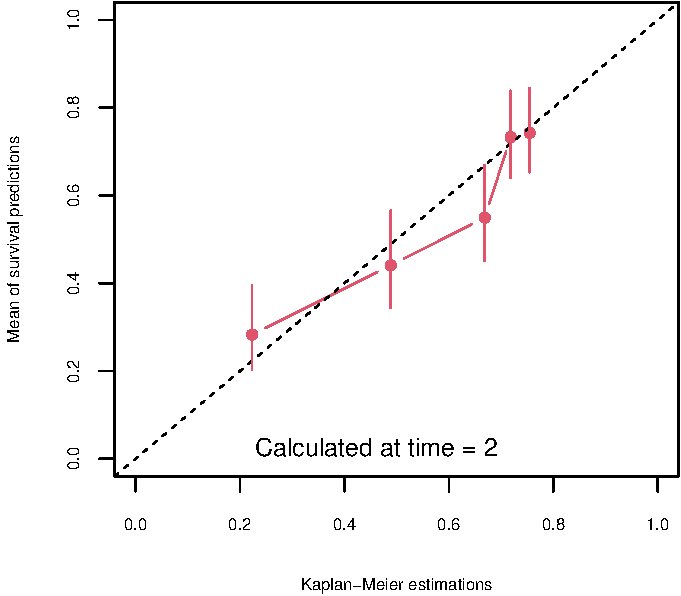
\includegraphics{RJ-2024-037_files/figure-latex/calibfig2-1.pdf}
\caption{\label{fig:calibfig2}Calibration plot at 2 years for the validation sample.}
\end{figure}

The \texttt{predict.sltime} function returns predicted survival probabilities. With this function, one can also investigate the calibration by comparing the mean of the predictions of the patients included in the validation sample and the observed relapse-free survival, as illustrated in Figure \ref{fig:calibfig3} (Appendix). The SL did not improve the discrimination capacities offered by the modified Rio score for a prognostic up to 2 years after the treatment initiation (Figure \ref{fig:rocfig2} in Appendix).

\hypertarget{conclusion}{%
\section{Conclusion}\label{conclusion}}

The present paper introduced the \pkg{survivalSL} package to estimate a SL from right-censored data, to evaluate its prognostic capacities, and to predict survival curves for new individuals. The solution allows a larger set of learners (models or algorithms) and several loss functions to estimate their contributions. The user can define a grid for estimating the hyperparameters by cross-validation, or even fix their values.

The simulation study illustrated the SL performances. More precisely, in a simple context (several independent covariates, respect of the log-linearity assumption, no interaction), its performances are equivalent to more simple PH models. In contrast, in a complex context, the performances of the simple PH models decreased, and the SL resulted in the best performances: both the means and the variances of the loss functions were comparatively small relative to other methods considered.

We illustrated the usage of the package for predicting the non-response of patients with multiple sclerosis treated with a first-line therapy. The S3 methods allow a simple evaluation of the prognostic capacities, which can be compared with those of existing scoring systems. In this simple application, comparable to the simple scenario of the simulation study, the SL did not result in higher prognostic capacities compared to the Elastic-net PH model or even the existing modified Rio score.

As machine learning is increasingly being used in predictive studies, we believe that our proposal will be useful for a large community of data analysts. Nevertheless, we can point to three limitations. Firstly, even if we considered many learners, the current version of the package does not allow the users to include their own algorithms or models. An important perspective of development is to integrate this functionality. Secondly, one can also note that the estimation of learners and their weights assume non-informative censoring. Introducing the inverse probability of censoring weighting (IPCW) method, to correct for dependent censoring, would be of great interest, but challenging for some learners such as neural networks or random survival forests.

\hypertarget{acknowledgments}{%
\section{Acknowledgments}\label{acknowledgments}}

We would like to thank David Laplaud, neurologist and specialist in multiple sclerosis, for his clinical advice. The OFSEP cohort is supported by a grant provided by the French National Agency for Research, within the framework of the Investments for Future (ANR-10-COHO-002), and by the Eugène Devic EDMUS Foundation against multiple sclerosis and the ARSEP Foundation.

\hypertarget{bug-reports}{%
\section{Bug reports}\label{bug-reports}}

To improve future versions of the package, you can report errors at the following address:

\texttt{https://github.com/chupverse/survivalSL/issues}

\newpage

\hypertarget{supplementary-materials}{%
\section{Supplementary materials}\label{supplementary-materials}}

\hypertarget{r-code-to-perform-the-simulations-of-the-simple-scenario}{%
\subsection{R code to perform the simulations of the simple scenario}\label{r-code-to-perform-the-simulations-of-the-simple-scenario}}

\begin{verbatim}
library(survivalSL)

# definition of the parameters related to the simulated data
n.valid <- 500 # sample size for validation
n.learn <- 500 # sample size for training

n <- n.valid + n.learn # overall sample size

max.time <- 50 # maximum follow-up time

mean.x <- 0; sd.x <- 1 # normal distribution of the quantitative predictors
proba.x <- .5 # proportion of the binary predictors

a <- 2; b <- .05 # Weibull baseline distribution of the PH model
beta <- c(log(1.8), log(1.8), log(1.3), 0, 0, 0) # regression coefficients

# simulation of  the training and validation samples
x1 <- rnorm(n, mean.x, sd.x)
x2 <- rbinom(n, 1, proba.x)
x3 <- rbinom(n, 1, proba.x)
x4 <- rnorm(n, mean.x, sd.x)
x5 <- rbinom(n, 1, proba.x)
x6 <- rbinom(n, 1, proba.x)
x <- cbind(x1, x2, x3, x4, x5, x6) # matrix of the potential predictors
  
u <- runif(n, 0, 1)
times <- 1/b*((-exp(-1*(x %*% beta))*(log(1-u)))**(1/a)) # time to event
  
censoring <- runif(n, min=0, max=max.time)
  
status <- ifelse(times <= censoring, 1, 0) # event status
obs.times <- ifelse(times <= censoring, times, censoring) # follow-up times
  
data <- cbind(obs.times, status, as.data.frame(x))
  
data.simul <- list(data[1:n.valid,], data[(n.valid+1):n,])

# definition of the grid search related to the hyperparameters

slres <- survivalSL(
  formula=Surv(obs.times, status) ~ x1 + x2 + x3 + x4 + x5 + x6,
  methods=c("LIB_COXen", "LIB_COXall", "LIB_RSF", "LIB_PLANN",
            "LIB_AFTgamma", "LIB_PHexponential"),
  metric="ibs",  data=data.simul[[1]], show_progress=FALSE, cv=10)

# loss functions estimated from training sample (Figure 1)
summary(slres) 

# from validation sample (Figure 1)
summary(slres, newdata=data.simul[[2]]) 
\end{verbatim}

\newpage

\hypertarget{r-code-to-perform-the-simulations-of-the-complex-scenario}{%
\subsection{R code to perform the simulations of the complex scenario}\label{r-code-to-perform-the-simulations-of-the-complex-scenario}}

\begin{verbatim}
library(survivalSL)

# definition of the parameters related to the simulated data
n.valid <- 500 # sample size for validation
n.learn <- 200 # sample size for training
n <- n.valid + n.learn # overall sample size

max.time <- 50 # maximum follow-up time

b0.t <- (-0.4) # intercept related to the predictors' distribution
b1.t <- log(2) # slope related to the predictors' distribution

a <- 2; b <- .05 # Weibull baseline distribution of the PH model
b1.o <- 0.69 # regression coefficients of the PH model

# simulation of  the training and validation samples
.x1 <- rnorm(n, 0, 1)
.x2 <- rnorm(n, b0.t + b1.t * .x1, 1)
.x3 <- rnorm(n, b0.t - b1.t * .x1 - b1.t * .x2, 1)
.x4 <- rnorm(n, b0.t + b1.t * .x3, 1)
.x5 <- rnorm(n, 0, 1)
.x6 <- 1 * (rnorm(n, 0, 1) > 0.66)
.x7 <- 1 * (rnorm(n, b0.t - b1.t * .x5, 1) > (-0.40))
.x8 <- rnorm(n, b0.t - b1.t * .x6, 1)
.x9 <- 1 * (rnorm(n, b0.t + b1.t * .x7, 1) > (-0.80))
.x10 <- rnorm(n, b0.t + b1.t * .x8, 1)
.x11 <- rnorm(n, 0, 1)
.x12 <- 1 * (rnorm(n, b0.t + b1.t * .x9, 1) > (0.84))
.x13 <- 1 * (rnorm(n, b0.t + b1.t * .x10, 1) > (-0.09))
.x14 <- rnorm(n, b0.t - b1.t * .x12 - b1.t * .x11, 1)
.x15 <- rnorm(n, b0.t - b1.t * .x12, 1)
.x16 <- 1 * (rnorm(n, 0, 1) > (-0.66))
.x17 <- 1 * (rnorm(n, b0.t - b1.t * .x16, 1) > (-0.92))
.x18 <- rnorm(n, 0, 1)
.x19 <- 1 * (rnorm(n, 0, 1) > (0.66))
.x20 <- 1 * (rnorm(n, 0, 1) > (0.66))
.x21 <- rnorm(n, 0, 1)
.x22 <- 1 * (rnorm(n, 0, 1) > (0.66))

data.obs <- data.frame(x1=.x1, x2=.x2, x3=.x3, x4=.x4, x5=.x5, x6=.x6,
    x7=.x7, x8=.x8, x9=.x9, x10=.x10, x11=.x11, x12=.x12, x13=.x13,
    x14=.x14, x15=.x15, x16=.x16, x17=.x17, x18=.x18, x19=.x19,
    x20=.x20, x21=.x21, x22=.x22)

bx <- b0.t + b1.t*data.obs$x1 - b1.t*data.obs$x3 + b1.t*data.obs$x5 -
  b1.t*data.obs$x7 + b1.t*data.obs$x9 - b1.t*data.obs$x11 +
  b1.t*data.obs$x13 - b1.t*data.obs$x15 - b1.t*data.obs$x17 +
  b1.t*data.obs$x19 - b1.t*data.obs$x21

pr.t <- (exp(bx) / (1 + exp(bx)))
data.obs$t.obs <- rbinom(n, 1, prob = pr.t)

bx <- b1.o*(data.obs$x2>-0.40) - b1.o*data.obs$x3 +
  b1.o*0.5*(data.obs$x3^2) + b1.o*data.obs$x6 + b1.o*data.obs$x7 +
  b1.o*data.obs$x10 + b1.o*0.5*(data.obs$x11^2) - b1.o*data.obs$x14 -
  b1.o*(data.obs$x15>-0.57) + b1.o*data.obs$x18 + b1.o*data.obs$x19 +
  b1.o*data.obs$t.obs + b1.o*0.5*data.obs$t.obs*data.obs$x18

u <- runif(n,0,1)
times <- 1/b*((-exp(-bx)*(log(1-u)))**(1/a))

censoring <- runif(n, min=0, max=max.time)
status <- ifelse(times <= censoring, 1, 0)
obs.time <- ifelse(times <= censoring, times, censoring)
  
data <- cbind(obs.time, status, data.obs)

data.simul <- list(data[1:n.valid,], data[(n.valid+1):n,])

slres <- survivalSL(
  formula=Surv(obs.time, status) ~ x1 + x2 + x3 + x4 + x5 + x6 + x7 + x8 + x9 + 
  x10 + x11 + x12 + x13 + x14 + x15 + x16 + x17 + x18 + x19 + x20 + x21 + x22,
  data=data.simul[[1]],  metric="ibs",  cv=10, show_progress=FALSE,
  methods=c("LIB_COXen", "LIB_COXall", "LIB_RSF", "LIB_PLANN",
            "LIB_AFTgamma", "LIB_PHexponential"))

# loss functions estimated from training sample (Figure 2)
summary(slres) 

# from validation sample (Figure 2)
summary(slres, newdata=data.simul[[2]]) 
\end{verbatim}

\hypertarget{fluctuation-of-the-results-according-to-the-seed}{%
\subsection{Fluctuation of the results according to the seed}\label{fluctuation-of-the-results-according-to-the-seed}}

We estimate three additional SL with 3 alternative initializations of the pseudo-random number generator.

\begin{verbatim}
sl2.1 <- survivalSL(formula=.f, data=dataTRAIN, metric="uno_ci",
      methods=c("LIB_COXen", "LIB_PHspline", "LIB_AFTggamma", "LIB_RSF"),
      cv=30, optim.local.min=TRUE, param.tune=.tune, show_progress=FALSE, seed=118)

sl2.2 <- survivalSL(formula=.f, data=dataTRAIN, metric="uno_ci",
      methods=c("LIB_COXen", "LIB_PHspline", "LIB_AFTggamma", "LIB_RSF"),
      cv=30, optim.local.min=TRUE, param.tune=.tune, show_progress=FALSE, seed=119)

sl2.3 <- survivalSL(formula=.f, data=dataTRAIN, metric="uno_ci",
      methods=c("LIB_COXen", "LIB_PHspline", "LIB_AFTggamma", "LIB_RSF"),
      cv=30, optim.local.min=TRUE, param.tune=.tune, show_progress=FALSE, seed=120)

rbind(
  seed.121 = summary(sl2,   newdata=dataVALID, method="sl", pro.time=2, digits=4),
  seed.122 = summary(sl2.1, newdata=dataVALID, method="sl", pro.time=2, digits=4),
  seed.123 = summary(sl2.2, newdata=dataVALID, method="sl", pro.time=2, digits=4),
  seed.124 = summary(sl2.3, newdata=dataVALID, method="sl", pro.time=2, digits=4))
\end{verbatim}

\begin{verbatim}
#>          metrics       method pro.time ROC.precision
#> seed.121 data.frame,10 "sl"   2        numeric,99   
#> seed.122 data.frame,10 "sl"   2        numeric,99   
#> seed.123 data.frame,10 "sl"   2        numeric,99   
#> seed.124 data.frame,10 "sl"   2        numeric,99
\end{verbatim}

\begin{verbatim}
rbind(
  seed.121 = sl2$weights$values,
  seed.122 = sl2.1$weights$values,
  seed.123 = sl2.2$weights$values,
  seed.124 = sl2.3$weights$values)
\end{verbatim}

\begin{verbatim}
#>               [,1]      [,2]       [,3]      [,4]
#> seed.121 0.2486286 0.3339517 0.17734499 0.2400747
#> seed.122 0.2713981 0.3002995 0.17599652 0.2523059
#> seed.123 0.1721614 0.5182388 0.08864614 0.2209536
#> seed.124 0.2427707 0.2397718 0.27035706 0.2471004
\end{verbatim}

\clearpage

\clearpage

\begin{figure}
\centering
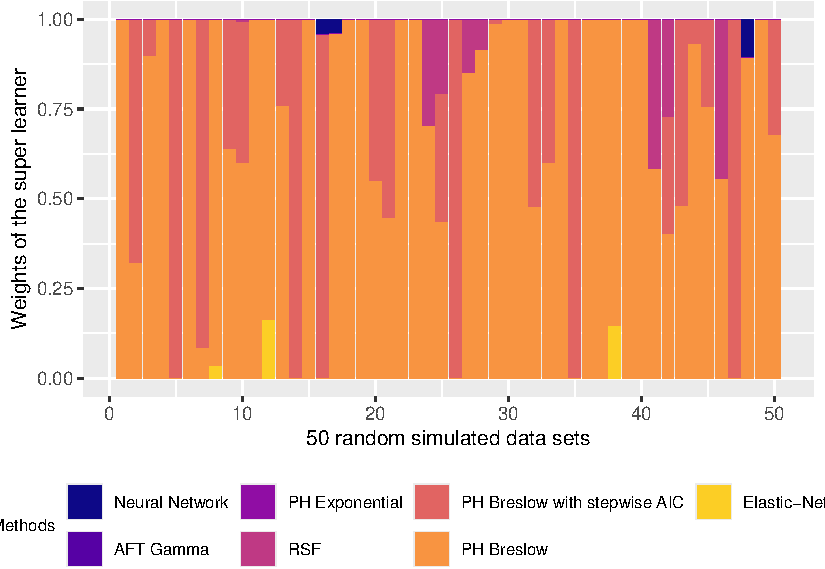
\includegraphics{RJ-2024-037_files/figure-latex/wscea-ggplot-1.pdf}
\caption{\label{fig:wscea-ggplot}Weight distribution among 50 randomly estimated super learners.}
\end{figure}

\clearpage

\begin{verbatim}
plot(survfit(Surv(time, event) ~ 1, data = dataVALID), 
     ylab="Disease progression free survival",
     xlab="Time after the first anniversary of the treatment in years",
     cex.lab = 0.8, cex.axis=0.8)

.pred.matrix <- predict(sl2, newdata=dataVALID,
                        newtimes = seq(0, 6, by=0.05))$predictions$sl

.pred <- apply(.pred.matrix, MARGIN=2, FUN="mean")

lines(x=seq(0, 6, by=0.05), y=.pred, col=2)

legend("bottomleft", c("Observed survival", "95% confidence interval",
        "Mean of the predictions"), col=c(1, 1, 2), lty=c(1,2,1), cex=0.8)
\end{verbatim}

\begin{figure}
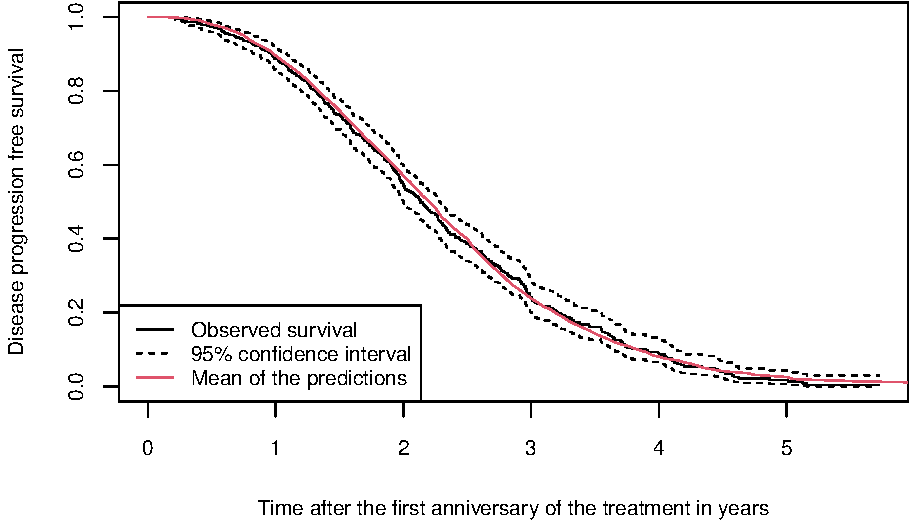
\includegraphics[width=1\linewidth]{RJ-2024-037_files/figure-latex/calibfig3-1} \caption{Observed relapse-free survival of the OFSEP validation sample (Kaplan-Meier estimator) compared to the mean of the individual predictions.}\label{fig:calibfig3}
\end{figure}

\clearpage

\begin{verbatim}
library("RISCA")

.pred <- predict(sl2, newdata=dataVALID)

dataVALID$sl <- 1 - .pred$predictions$sl[,sum(.pred$times<2)]

roc.sl <- roc.time(times="time", failures="event", variable="sl",
                  confounders=~1, data=dataVALID, pro.time=2,
                  precision=seq(0.1, 0.9, by=0.01)) 
# Note: “confounders=~1” for usual time-dependent ROC curves,
# i.e., without considering confounder (doi:10.1177/0962280217702416)

roc.rio <- roc.time(times="time", failures="event", variable="rio",
                   confounders=~1, data=dataVALID, pro.time=2)

plot(roc.sl, col=2, type="l", xlab="1-Specificity", ylab="Sensitivity",
     cex.lab=0.8, cex.axis=0.8)

points(x=1-roc.rio$table$sp, y=roc.rio$table$se, col=4)

legend("bottomright", legend=
  paste("AUC =", round(roc.sl$auc, 3)), cex=0.8 )
\end{verbatim}

\begin{figure}
\centering
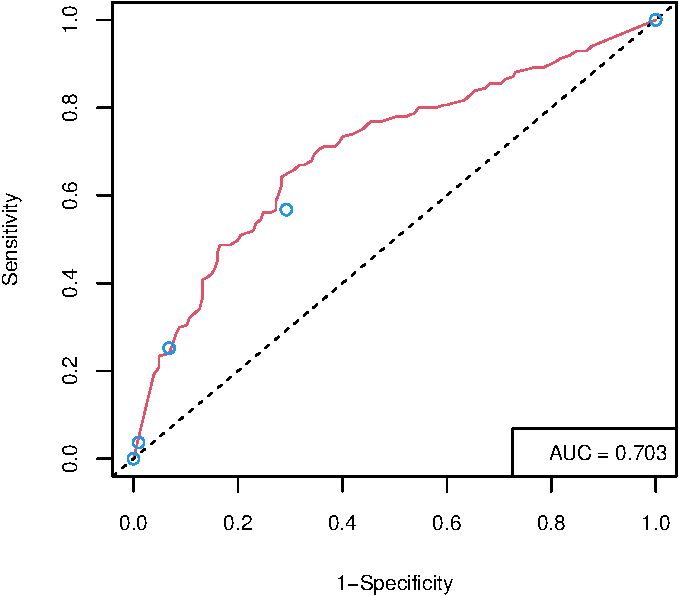
\includegraphics{RJ-2024-037_files/figure-latex/rocfig2-1.pdf}
\caption{\label{fig:rocfig2}ROC curve of the SL (line in red) compared to the sensitivity and specificity of the modified Rio score (points in blue) for a prognostic up to 2 years in the OFSEP validation sample.}
\end{figure}

\clearpage

\bibliography{Survsuperlearner.bib}

\address{%
Camille Sabathe\\
Nantes University, INSERM U1246 SPHERE, France\\%
22, Bd Benoni Goullin, F-44200 Nantes\\
%
%
\textit{ORCiD: \href{https://orcid.org/0000-0001-9353-691X}{0000-0001-9353-691X}}\\%
\href{mailto:camille.sabathe@univ-nantes.fr}{\nolinkurl{camille.sabathe@univ-nantes.fr}}%
}

\address{%
Yohann Foucher\\
University and Hospital of Poitiers, CIC INSERM 1402\\%
2, rue de la Miletrie, F-86000 Poitiers, France\\
%
%
\textit{ORCiD: \href{https://orcid.org/0000-0003-0330-7457}{0000-0003-0330-7457}}\\%
\href{mailto:yohann.foucher@univ-poitiers.fr}{\nolinkurl{yohann.foucher@univ-poitiers.fr}}%
}
